
\section{NICAM is}

\NICAM (Nonhydrostatic Atmospheric ICosahedral Model) is an global
atmospheric model for the climate study, mainly developed by Japan Agency for Marine-Earth
Science and Technology (JAMSTEC), Atmosphere And Ocean Research Institute (AORI) of
U-Tokyo, and RIKEN.
Since aiming high-resolution global atmospheric simulation, this model has several features, such as;

\begin{itemize}
 \item cloud-system resolving approach,
 \item icosahedral grid system,
 \item targetting massively parallel supercomputer.
\end{itemize}

This manual describes the overview of \NICAM and each kernel program briefly.
For the details of \NICAM , see
\cite{Tomita:2004kf},
\cite{Satoh:2008fb},
\cite{Satoh:2014dm},
 etc.

\section{Governing equations and the coordinate system}

% Tomita_etal_2008_SIAM

The governing equations of \NICAM are based on a fully compressible
non-hydrostatic system, including acoustic waves, fast gravity waves and
slow gravity waves.
%
As a coordinate system, \NICAM uses the Cartesian coordinate in
3-dimensional space.
%
Introducing an orthogonal basis $\{\bm{e_1}, \bm{e_2}, \bm{e_3}\}$, that
is independent of space with $\bm{e_3}$ being in the same direction as
the angular velocity of the Earth, a 3-dimensional velocity $\bm{v}$ on the Earth's surface
with reference to the bases $\bm{e_1}$, $\bm{e_2}$ and $\bm{e_3}$ has
the three components $\{v_1, v_2, v_3\}$.
%
Furthermore, the velocity $\bm{v}$ is sometimes separated into a ``horizontal element''
and ``vertical element'' of that vector quantity.
This treatment is useful in the horizontal-explicit-vertical-implicit scheme, which is used in NICAM.
The wind component of radial direction is separated from $\bm{v}$ and named as a vertical wind $w$.
The residual is horizontal wind and expressed as $\bm{v}_h$ = $\{v_x, v_y, v_z\}$.

The 3-dimensional Cartesian notations are used mainly in dynamical core of NICAM.
In the physics package, more general wind velocity notations are used:
the zonal wind $u$, meridional wind $v$, and vertical wind $w$.
the same velocity $\bm{v}$ can be denoted as
\begin{equation}
 \bm{v} = u \bm{\hat{i}}  + v \bm{\hat{j}} + w \bm{\hat{k}}
\end{equation}
where $\bm{\hat{i}}$, $\bm{\hat{j}}$, and $\bm{\hat{k}}$ are unit vectors in the
longitudinal, latitudinal direction, and outward unit vector in the
vertical direction at the given point on the sphere, respectively.

%
% Tomita_etal_2010_ecmwf
%
\NICAM have a switch for the shallow-atmosphere approximation.
The shallow-atmosphere approximation has inconsistency in the conservation of absolute angular momentum
without several metric terms and the vertical Coriolis term.
%
\NICAM introduces a ``deep'' factor
%
\begin{equation}
 \gamma \equiv r/a
\end{equation}
%
where $r$ is the distance from the center of the Planet,
and $a$ is the radius of the Planet at sea level.
If we use the shallow-atmosphere approximation, $\gamma$ is set to 1.

For vertical coodinate, \NICAM employs a terrain-following coodinate with
the following metrics:
%
\begin{equation}
 \xi = \frac{\xi_T(z-z_s)}{z_T - z_s}, \qquad
  G^{1/2} \equiv (\frac{\partial z}{\partial \xi})_\text{h},  \qquad
  \bm{G^{z}} \equiv \nabla_\text{h0} \xi = -\frac{\tilde{\nabla}_\text{h0} z}{G^{1/2}}
\end{equation}
%
where $z_T$ is the top of the model domain, $z_s$ is the surface height,
$(\partial/\partial \xi)_\text{h}$ denotes the derivative along the vertical
direction,
and $\tilde{\nabla_\text{h0}}$ denotes the spherical gradient operator along
a constant $\xi$ plane at sea level.
Since $G^{1/2}\gamma^{2}$ is the factor of volume against the surface,
\NICAM treats the prognostic variable multiplied by this factor.
%
For example, the perturbation density is
$R = (\rho-\rho_\text{ref})G^{1/2}\gamma^2 $, %
where subscript $\text{ref}$ means the hydrostatic reference state,
the horizontal and vertical momentum are
$\bm{V}_h = \rho G^{1/2}\gamma^2 \bm{v}_h$ and
$W = \rho G^{1/2}\gamma^2 w$, respectively,
the internal energy is
$E = \rho G^{1/2}\gamma^2 e$.

The governing equations are as follows:

\begin{align}
 & \DP{R}{t} + \tilde{\nabla}_\text{h0}\cdot\frac{\bm{V}_h}{\gamma} +
 \DP{}{\xi} \left(\frac{\bm{V}_h}{\gamma}\cdot\bm{G^z} + \frac{W}{G^{1/2}}
 \right) = 0,%
 \\
 & \DP{\bm{V}_h}{t} + \tilde{\nabla}_h \frac{P}{\gamma} +
 \DP{}{\xi}\left(\bm{G^z}\frac{P}{\gamma}\right)
 = -\tilde{\bm{A}}_h - \tilde{\bm{C}}_h,%
 \\
 & \DP{W}{t} + \gamma^2 \DP{}{\xi}\left(\frac{P}{G^{1/2}\gamma^2}\right)
 + Rg = (-\tilde{A}_z -\tilde{C}_z ),%
 \\
 & \DP{E}{t} + \tilde{\nabla}_\text{h0} \cdot
 \left(h\frac{\bm{V}_h}{\gamma}\right)
 + \DP{}{\xi}\left[h\left(\frac{\tilde{\bm{V}}_h}{\gamma}\cdot\bm{G^z} + \frac{W}{G^{1/2}}
\right)
 \right]\nonumber\\
& -\left[\bm{v}_h \cdot \left(\tilde{\nabla}_\text{h0}\frac{P}{\gamma} + \DP{}{\xi}\left(\bm{G^z}\frac{P}{\gamma}
\right)
\right)
+ w \left(\gamma^2 \DP{}{\xi}\left(\frac{P}{G^{1/2}\gamma^2}
\right)
+Rg
\right)
\right] + Wg = \tilde{Q}_{heat},
\end{align}
%
where $P = (p-p_\text{ref})G^{1/2}\gamma^2$ is the perturbation
pressure,
$h$ is the enthalpy,
$g$ is the gravitational acceleration,
and $\tilde{Q}_\text{heat}$ is the heating rate.
%
$\tilde{\bm{A}}$($=\tilde{\bm{A}_h}+\tilde{A}_z\bm{k}$) and
$\tilde{\bm{C}}$($=\tilde{\bm{C}_h}+\tilde{C}_z\bm{k}$) are
momentum advection term and Coriolis term, respectively.
%
Using an orthogonal basis $\{\bm{e}_1,\bm{e}_2,\bm{e}_3,\}$,
which is independent of space with $\bm{e}_3$ being in the same
direction as the angular velocity of the Planet $(0,0,\Omega)$.
%
Similarly, the three-dimensional velocity $\bm{v}$ is shown as
$(v_1, v_2, v_3)$ with regard to the basis $\bm{e_1}$, $\bm{e_2}$ and
$\bm{e_3}$, respectively.
%
Using these $\tilde{\bm{A}}$ and $\tilde{\bm{C}}$ can be expressed as
%
\begin{align}
 \tilde{\bm{A}} &\equiv \sum^3_{i=1} \left[\tilde{\nabla}_\text{h0}\cdot\left(v_i\frac{\bm{V}_h}{\gamma}\right)
+\DP{}{\xi}\left[v_i\left(\frac{\bm{V}_h}{\gamma}\cdot\bm{G^z} + \frac{W}{G^{1/2}}
\right)
\right]
 \right]\bm{e}_i,
\\
 \tilde{\bm{C}} &\equiv 2\Omega\rho G^{1/2}\gamma^2( -v_2\bm{e}_1 +v_1\bm{e}_2 ).
\end{align}

\section{Time integration}\label{s:time_integration}

The set of governing equations that \NICAM uses is an elastic system, so
it contains all the waves, especially acoustic waves, high-frequency
gravity waves and the Lamb waves.
These are called as the ``fast modes''.
The governing equations can be described schematically as

\begin{equation}
 \frac{\partial\Psi}{\partial t} - F = S,
\end{equation}
%
where $\Psi$, $F$ and $S$ represent the prognostic variable, the
fast-mode term, and the slow-mode term, respectively.
%
For small time step integration a forward-backward scheme based on the
HEVI (horizontally explicit and vertically implicit) method is used,
while for large time step integration the second- or third-stage
Runge-Kutta method \citep{Wicker:2002jd} is used.
%
This scheme treats fast waves implicitly in the vertical direction
only, and Helmholtz equation is one-dimensional and can be solved
directly as by the tridiagonal matrix solver (See \autoref{s:vert_coord}).
%
The time step is restricted by the horizontal grid space, explicit
scheme is used in that direction.
%
The fast-mode term are evaluated at every small time step $\Delta \tau$,
and the slow-mode term are evaluatied at larger time step $\Delta t$
(\autoref{f:temporal_integration}).
%


\begin{figure}[tb]
\centering
 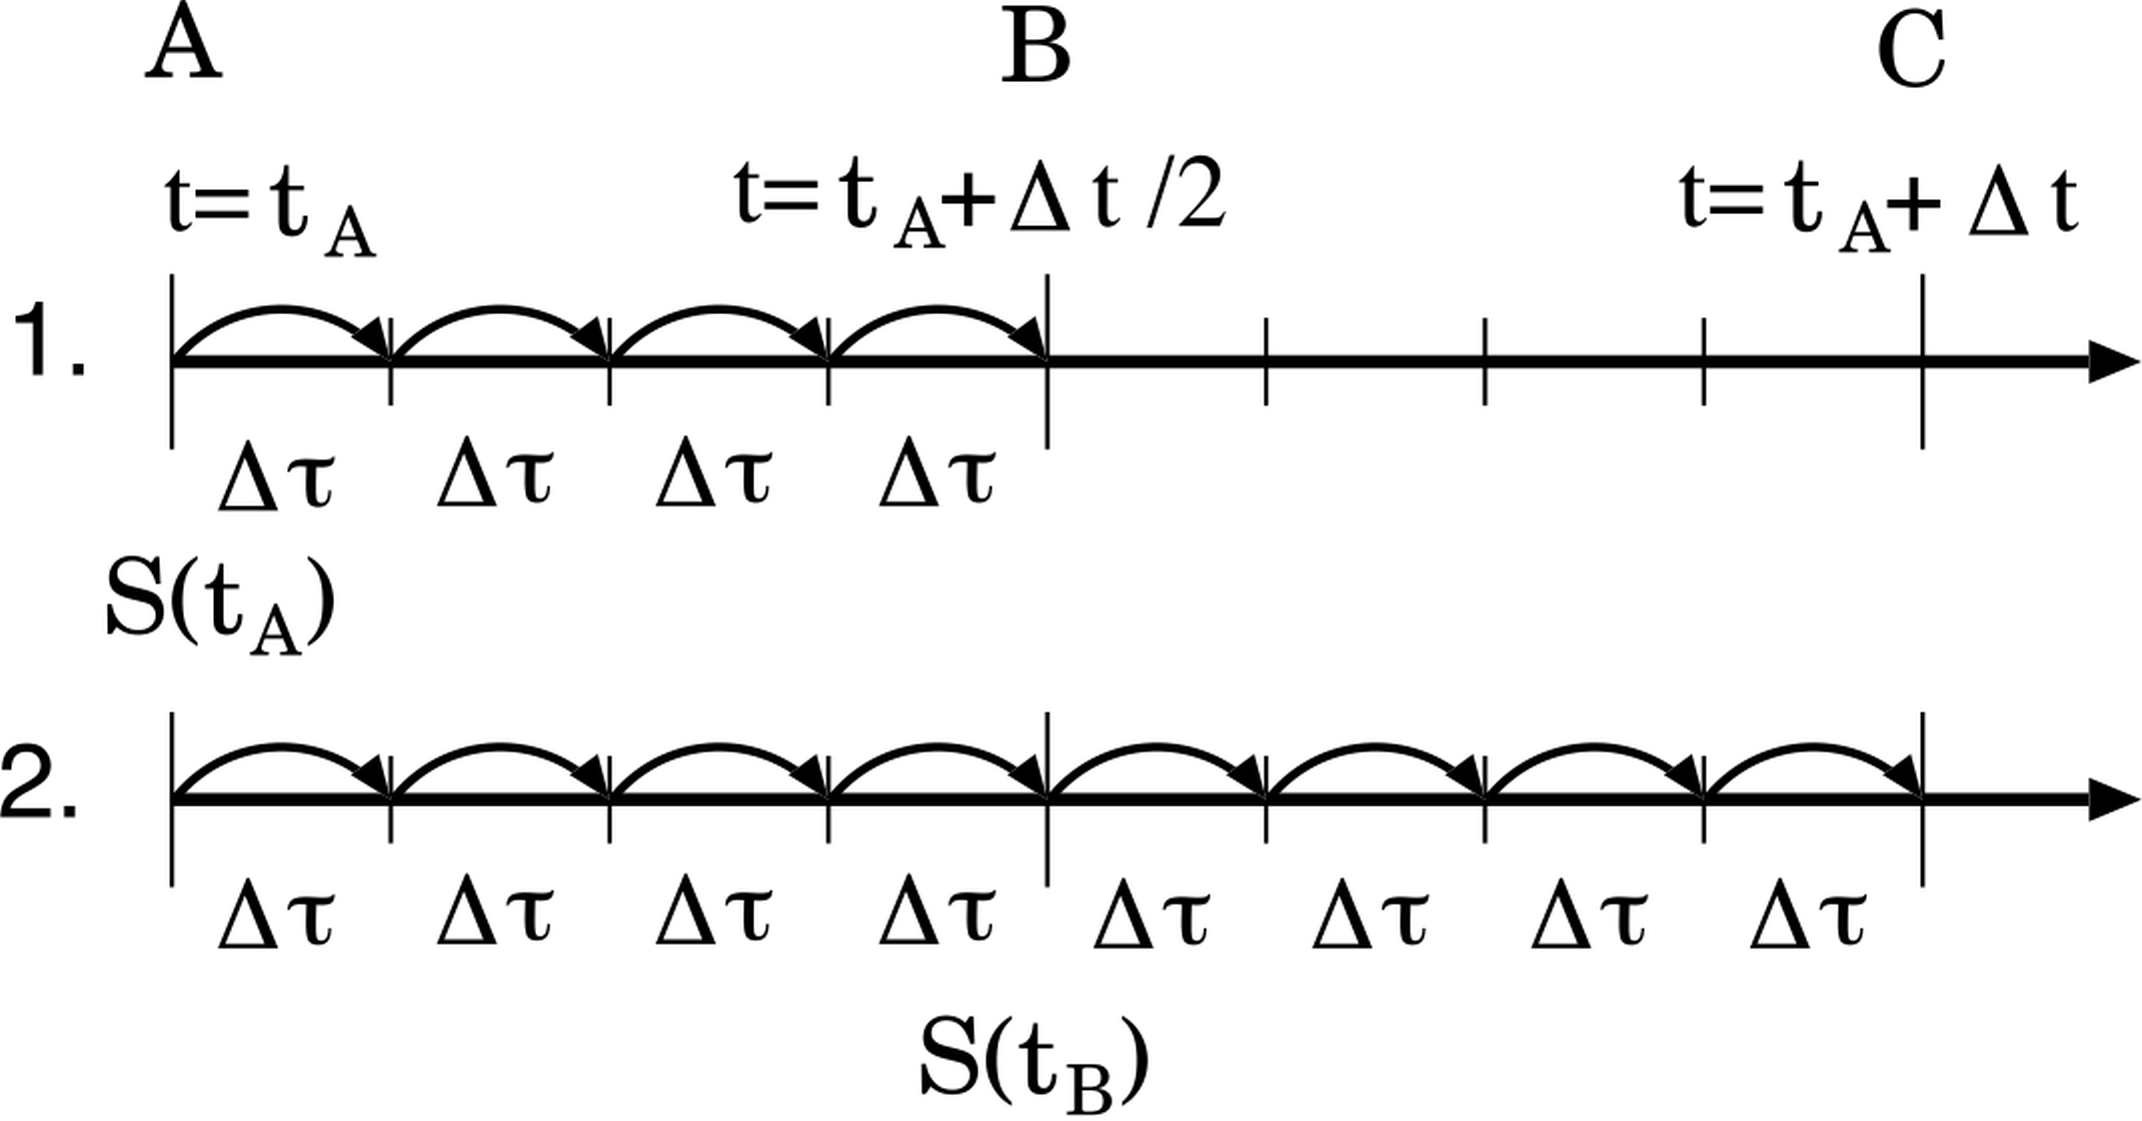
\includegraphics[scale=.3]{figs/Tomita1-20-0.png}
\caption{Schematic figure of temporal integration.}
\label{f:temporal_integration}
\end{figure}

If $\Psi$ at $t = t_A$ is given, the slow-mode tendency $S(t_A)$ can be
evaluated.
%
The variable is integrated from $t_A$ to $t_B (> t_A)$ using
%
$S(t_A) + F(t_A + m\Delta\tau)$ as the forcing function at $t=t_A +
m\Delta\tau$,
where $F(t_A + m\Delta\tau)$ is the fast-mode tendency being updated at
every small step and $m$ is the index of small time steps.
%
Repeating integration with this small step, the temporary value of the
prognostic variable $\Psi^*$ at $t_B$ can be obtained.
%
The slow-mode tendency $S(t_B)$ is evaluated using this value.
%
Finally, integrated variable $\Psi$ at $t=t_C(>t_B)$ is calcurated by
$S(t_B) + F(t_A + m\Delta\tau)$.



\section{Icosahedral grid and ``glevel''}\label{s:ico_grid_glevel}

To overcome the pole problem which old-fashioned global models have,
\NICAM uses the icosahedral grid system.
In this grid system, grid points are distributed quasi-homogeneously on
the sphere.
%
The icosahedral grid can be constructed by a recursive division method
which is similar to that of \cite{Stuhne:1996fr}.
%
The grid resolution obtained by $i$-th dividing operation is called
``glevel-$i$''.
%
First, vertices of the spherical icosahedron construct glevel-0 (
\autoref{f:glevel_0}).
%
By connecting the midpoint of each edge of the triangles, the next finer
grid glevel-1 is generated as \autoref{f:glevel_1}.
%
Doing the same procedure, glevel-2 is
generated(\autoref{f:glevel_2}).
%
For example, \autoref{f:glevel_5} shows the
glevel-5 grid.

\begin{figure}[tb]
\centering
\begin{subfigure}{.32\textwidth}
\centering
 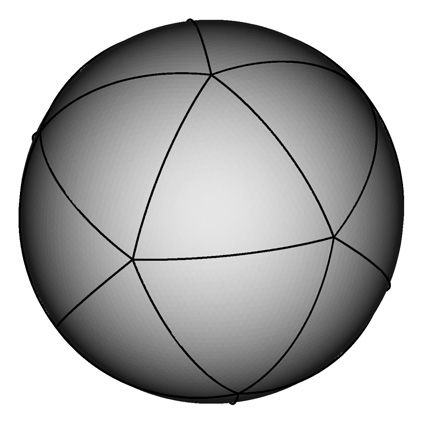
\includegraphics[width=\textwidth]{figs/Tomita_etal_2008_SIAM-7-0.png}
\caption{glevel=0}\label{f:glevel_0}
\end{subfigure}
\begin{subfigure}{.32\textwidth}
\centering
 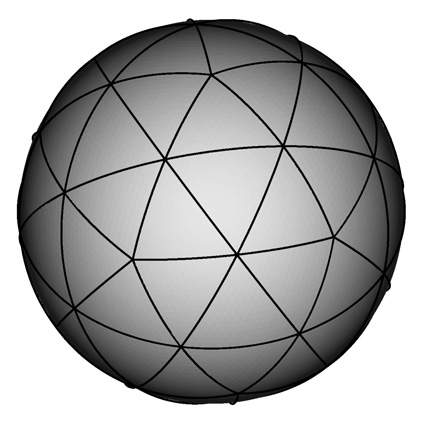
\includegraphics[width=\textwidth]{figs/Tomita_etal_2008_SIAM-7-1.png}
\caption{glevel=1}\label{f:glevel_1}
\end{subfigure}
\begin{subfigure}{.32\textwidth}
\centering
 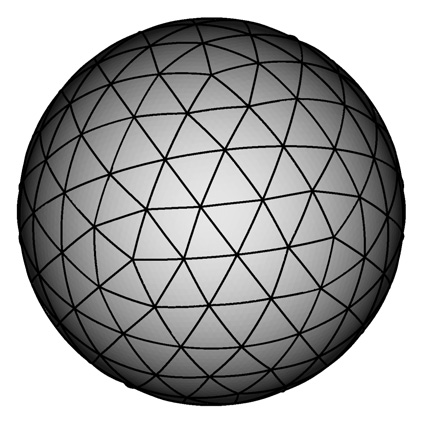
\includegraphics[width=\textwidth]{figs/Tomita_etal_2008_SIAM-7-2.png}
\caption{glevel=2}\label{f:glevel_2}
\end{subfigure}
\caption{The method of horizontal grid refinement.}\label{f:horiz_grid_refinement}%\label{195813_22Oct17}
\end{figure}

\begin{figure}[tb]
\centering
 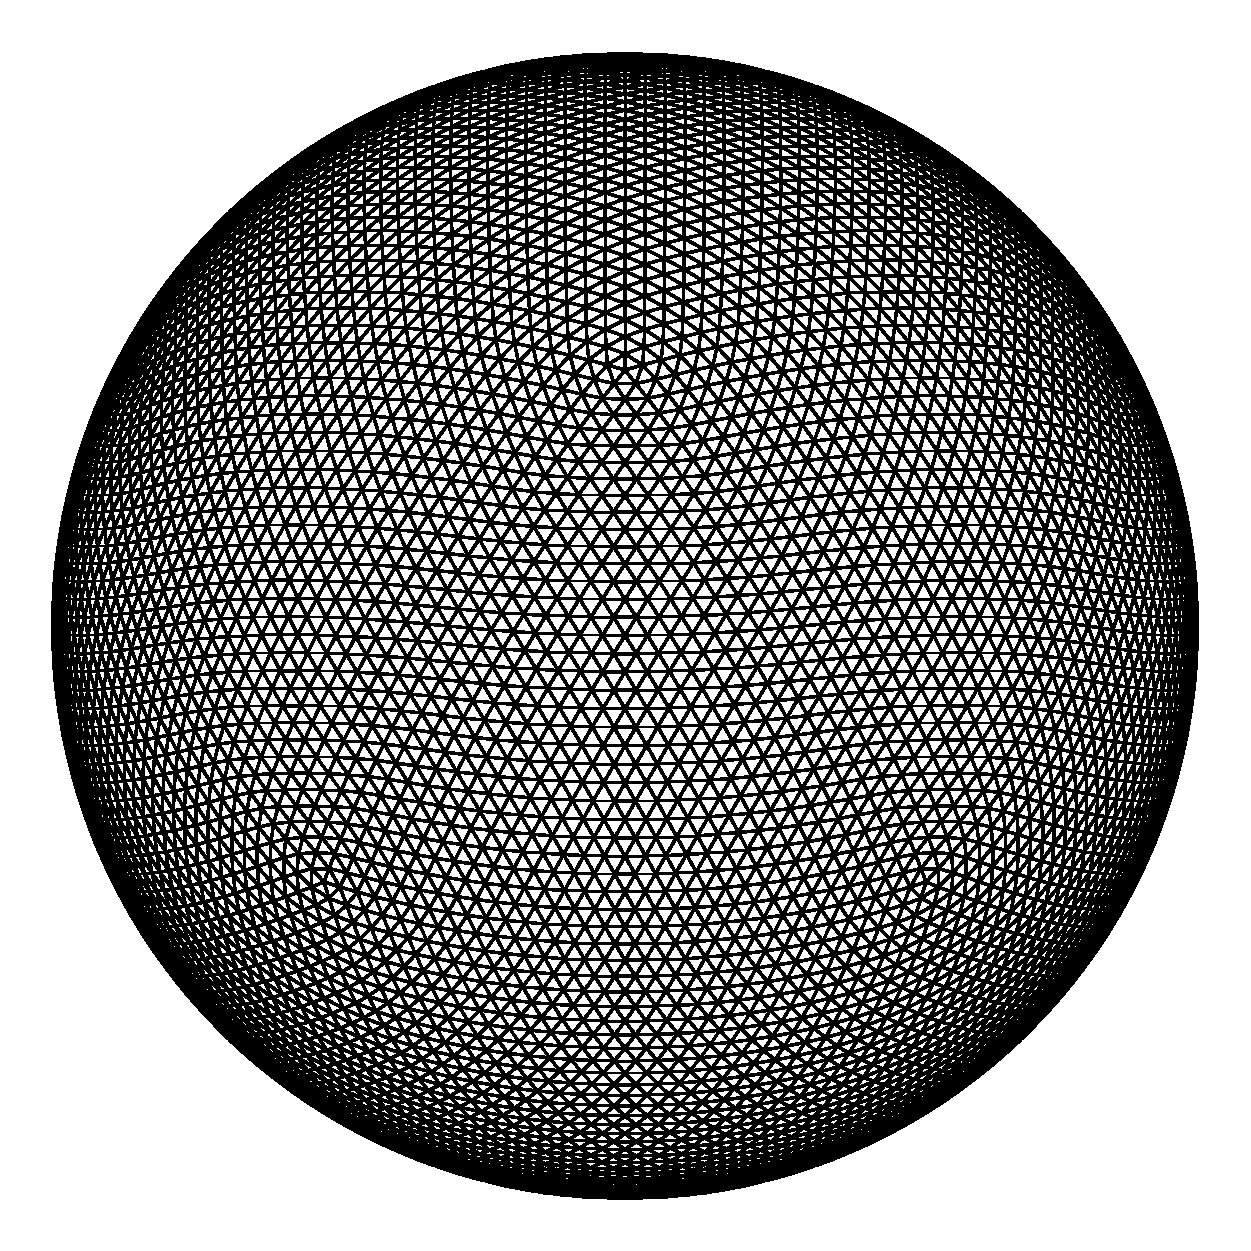
\includegraphics[scale=.25]{figs/Tomita1-26-0.png}
 \caption{The icosahedral grid with glevel-5}
 \label{f:glevel_5}
\end{figure}


All the variables are defined at the vertices of triangular grid
elements.
%
This arrangement is categorized into the Arakawa-A type grid.
%
The control volume is defined as the polygon constructed by connecting
the gravitational centers of neighboring triangular grid elements.
%
The shape of control volume is hexagon, as shown in
\autoref{f:control_volume}, except that it is pentagon at only twelve points
inherited from the original icosahedron.

\begin{figure}[tb]
 \centering
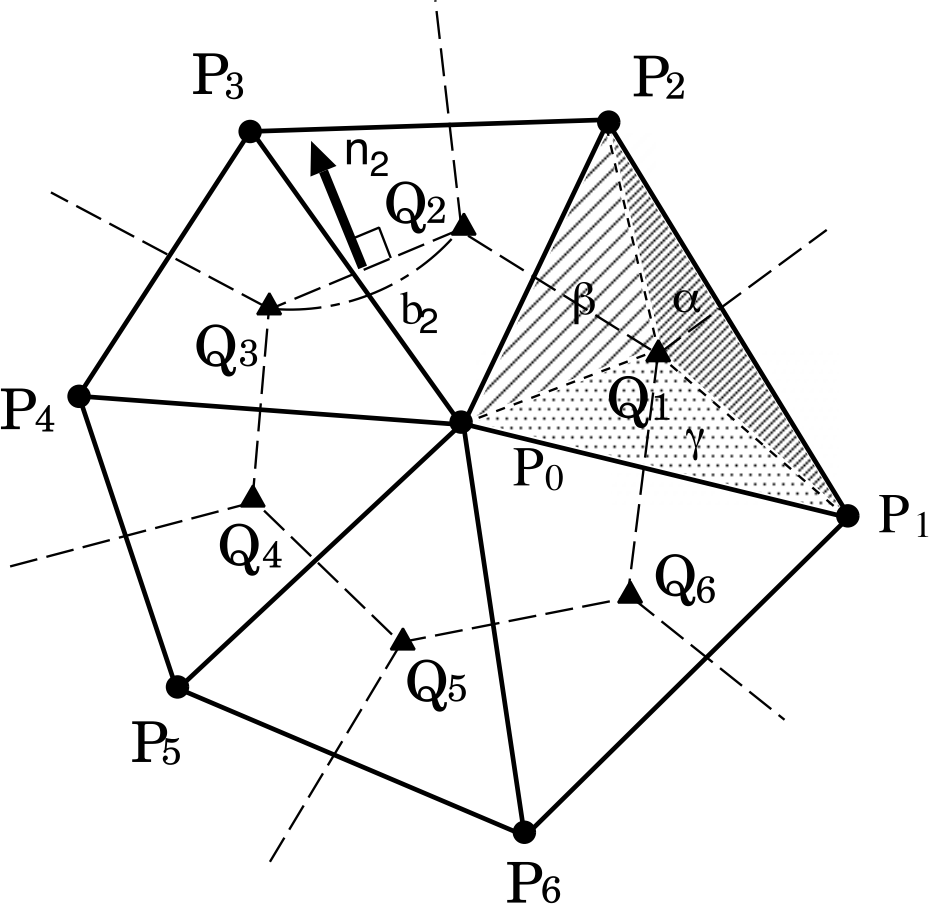
\includegraphics[scale=0.7]{figs/Tomita1-27-0.png}
 \caption{Schematic figure of control volume. \citep{Tomita:2008jc}}
 \label{f:control_volume}
\end{figure}


\NICAM adopts the finite volume method for the discretization of
differential operators.
%
In \autoref{f:control_volume}, some vector $\bm{u}$
at the vertices of control volume $Q_i$ are calculated by interpolation
as\footnotemark
%
\footnotetext{$P_{i+1}$ should be $P_{1+\text{mod}{(i,6)}}$, and the same hereinafter.}
%
\begin{equation}
 \bm{u} (Q_i) \simeq
 \frac{\alpha \bm{u}(P_0) + \beta \bm{u}(P_i) + \gamma \bm{u}(P_{i+1})}
      {\alpha + \beta + \gamma} ,\label{e:u_Q_i}
\end{equation}
%
where $\alpha$, $\beta$ and $\gamma$ are the areas of the triangle
$Q_i P_i P_{i+1}$, $Q_0 P_{i+1} P_0$ and $Q_i P_0 P_i$, respectively.
%
The number 6 is replaced with 5 at the pentagonal control volumes for
the singular points.

The divergence is calculated from the Gauss theorem as
%
\begin{equation}
 \nabla \cdot \bm{u}(P_0) \simeq \frac{1}{a(P_0)} %
  \sum^{6}_{i=1} b_i \frac{\bm{u}(Q_i)+\bm{u} (Q_{i+1})}{2} \cdot
  \bm{n}_i,\label{e:nabla_u_P_0}
\end{equation}
%
where $b_i$ and $\bm{n}_i$ denote the geodesic arc length of
$Q_i Q_{i+1}$ and the outward unit vector normal to this arc at the
midpoint of $Q_i Q_{i+1}$.
%
$a(P_0)$ is the area of control volume at the point $P_0$.
%
More than that, \autoref{e:nabla_u_P_0} can be rewritten as a
linear combination:
%
\begin{equation}
 \nabla \cdot \bm{u} (P_0) = \sum^{6}_{i=1} \bm{c}_i \cdot \bm{u}(P_i)\label{e:nabla_u_P_0_eq}
\end{equation}
%
where $\bm{c}_i$ are constant vector coefficients which can be
pre-calculated once and stored for subsequent use.
%
In \autoref{e:nabla_u_P_0_eq}, the number of addition and
multiplication is the same, this formulation is preferable for the CPU
which has FMA.



The gradient operator to an arbitrary variable $\phi$ is calculated as

\begin{equation}
 \nabla \phi(P_0) \simeq
  \frac{1}{a(P_0)}
  \sum^{6}_{i=1} b_i \frac{\phi(Q_i) + \phi(Q_{i+1})}{2} \bm{n}_i
  - \frac{\phi_0}{a(P_0)} \sum^{6}_{i=1} b_i \bm{n}_i,\label{e:nabla_phi_P_0}
\end{equation}
%
where $\phi(Q_i)$ is interpolated by the similar way to the
\autoref{e:u_Q_i}.
%
This scheme given as \autoref{e:nabla_phi_P_0} generates the
vertical component because the allocation points are on the sphere.
%
In practice, the vertical component is removed after the operation of
\autoref{e:nabla_phi_P_0}.


More precisely, \NICAM used modified icosahedoral grid by using spring dynamics in order to avoid
severe problems on the numerical accuracy and stability.
See \cite{Tomita:2001id} for the details.
%


\section{Upwind-Biased Advection Scheme}\label{s:upwind_scheme}

\NICAM uses an upwind-biased advection scheme for icosahedral grid
derived by \cite{Miura:2007bs}.
%
\autoref{f:2007mwr2101_1-0} (a) shows arrangement of distorted hexagonal
cells. Computational nodes are $\bm{P}_i(i=0,2,...,6)$, hexagonal cell
corners are $\bm{Q}_i$, center of hexagonal cell faces are $\bm{R}_i$,
lengths of hexagonal cell faces are $l_i$, and unit vectors normal to
cell faces are $\bm{n}_i$.
%
\autoref{f:2007mwr2101_1-0} (b) shows schematic of the area swept by the
arc $\bm{Q}'_i\bm{Q}'_{i+1}$ during a time interval.
%
Here we assumes that the arc $\bm{Q}'_i\bm{Q}'_{i+1}$ at time $t$
moves with a constant velocity $\bm{v_R}^{t+\Delta t/2}$
and concides with the arc $\bm{Q}_i\bm{Q}_{i+1}$ at time $t+\Delta t$.
%
The total amount of flux through the edge $\bm{Q}_i\bm{Q}_{i+1}$
during the time interval $\Delta t$ is approximated by the amount of a
tracer inside the parallelogram
$\bm{Q}'_i\bm{Q}'_{i+1}\bm{Q}_{i+1}\bm{Q}_i$,
%
Profiles of $\rho$ and $q$, he density and the
tracer mixing ratio, respectively, inside this parallelogram can be
approximated by two-dimensional linear surface.
%
Then the amount of a tracer inside this parallelogram is
%
\begin{equation}
\rho_{\bm{R}_i} q_{\bm{R}_i}
 = \frac{\int_{S_i} \rho q \ \mathrm{d}S}
         {S_i}
 = \rho_{\bm{C}_i} q_{\bm{C}_i},
\end{equation}
%
where $S_i$ and
$\bm{C}_i$ denotes the area and the mass centroid of this parallelogram, respectively.
%
Similarly, the continuity equation will yield
%
\begin{equation}
 \rho_{\bm{R}_i} = \rho_{\bm{C}_i}.
\end{equation}
%
Thus,
%
\begin{equation}
 q_{\bm{R}_i} = q_{\bm{C}_i}.
\end{equation}
%
The position of $\bm{C}_i$ can be computed as
%
\begin{equation}
\bm{C}_i = \bm{R}_i - v_{\bm{R}_i}^{t+\Delta t/2} \frac{\Delta t}{2}.
\end{equation}
%
Linear surfaces inside the parallelogram can be approximated by nodal
values and gradients at a computational node that shares the cell face
and is on the upwind side of the cell face.
%
See \cite{Miura:2007bs} for more details.

\begin{figure}[htbp]
\centering
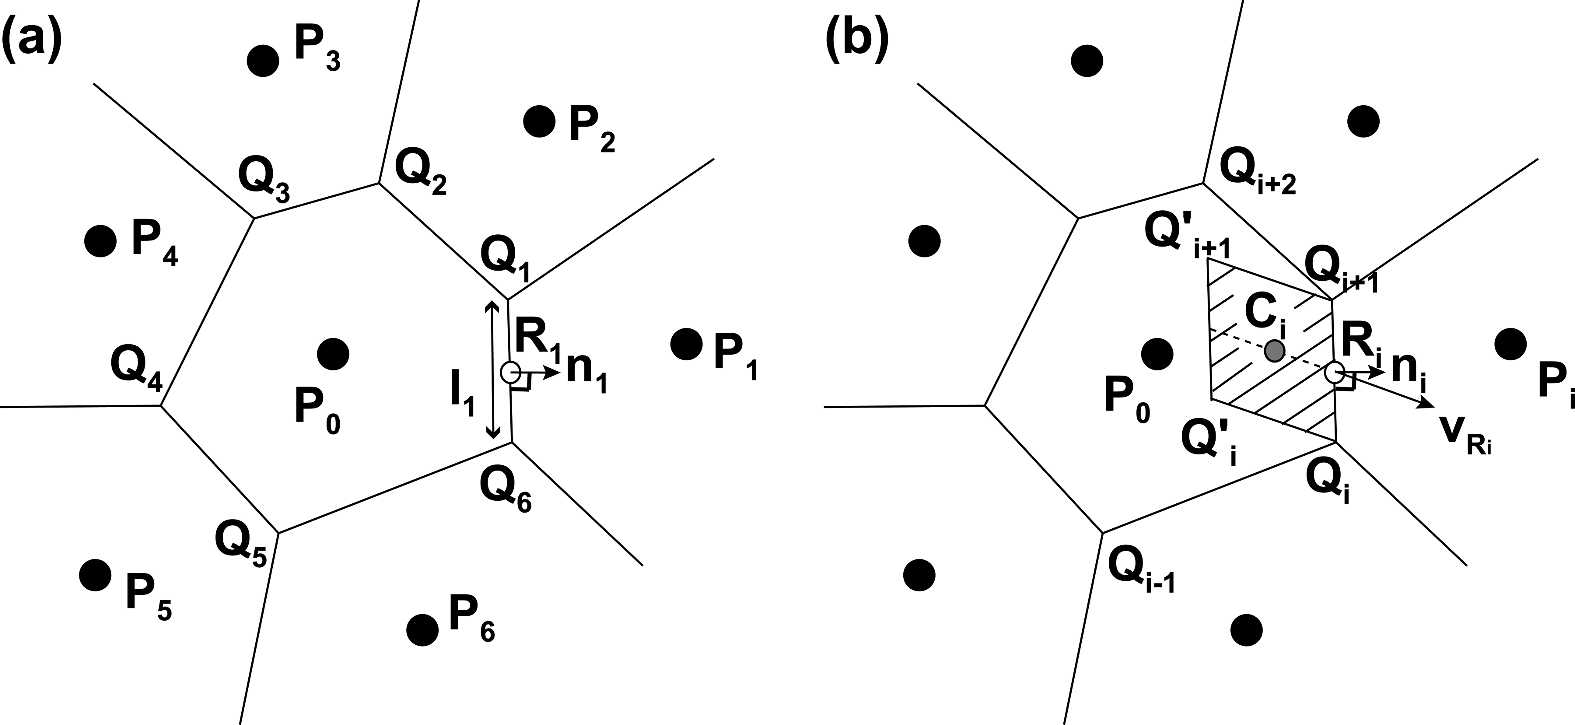
\includegraphics[scale=.3]{figs/2007mwr2101_1-0.png}
 \caption{%
(a) Arrangement and notation of distorted hexagonal cells.%
(b) Schematic of the area swept by the arc $\bm{Q}'_i \bm{Q}'_{i+1}$ during a time interval.%
}\label{f:2007mwr2101_1-0}
\end{figure}


\section{Vertical coordinate and discretization}\label{s:vert_coord}

\NICAM uses the Lorenz grid for the vertical grid configuration as shown
in \autoref{f:vert_grid_config},
where $W$ (vertical velocity with metrics) is defined at the
half-integer levels and the other variables are defined at the integer
levels.
%
This model allows the grid stretching in the $\xi$ coordinate as show in
\autoref{f:vert_grid_config}.
%
The integer levels are located at the mid-point of the upper and lower
half-integer levels.
%
The linear interpolation is used to obtain the values at the
half-integer levels from the values at the integer levels, and vice
versa:
%
\begin{align}
 \phi_{k+1/2} &= a_{k+1/2}\, \phi_{k+1} + b_{k+1}\,\phi_k,\\
 \phi_k       &= c_k \, \phi_{k+1/2} + d_k \, \phi_{k-1/2},
\end{align}
%
where
%
\begin{align}
 a_{k+1/2} &= \frac{\xi_{k+1/2} - \xi_k}{\xi_{k+1}-\xi_k},\\
 b_{k+1/2} &= 1 - a_{k+1/2} ,\\
 c_k       &= \frac{\xi_k - \xi_{k-1/2} }{\xi_{k+1/2} - \xi_{k-1/2}},\\
 d_k       &= 1 - c_k.\\
\end{align}


\begin{figure}[tb]
\centering
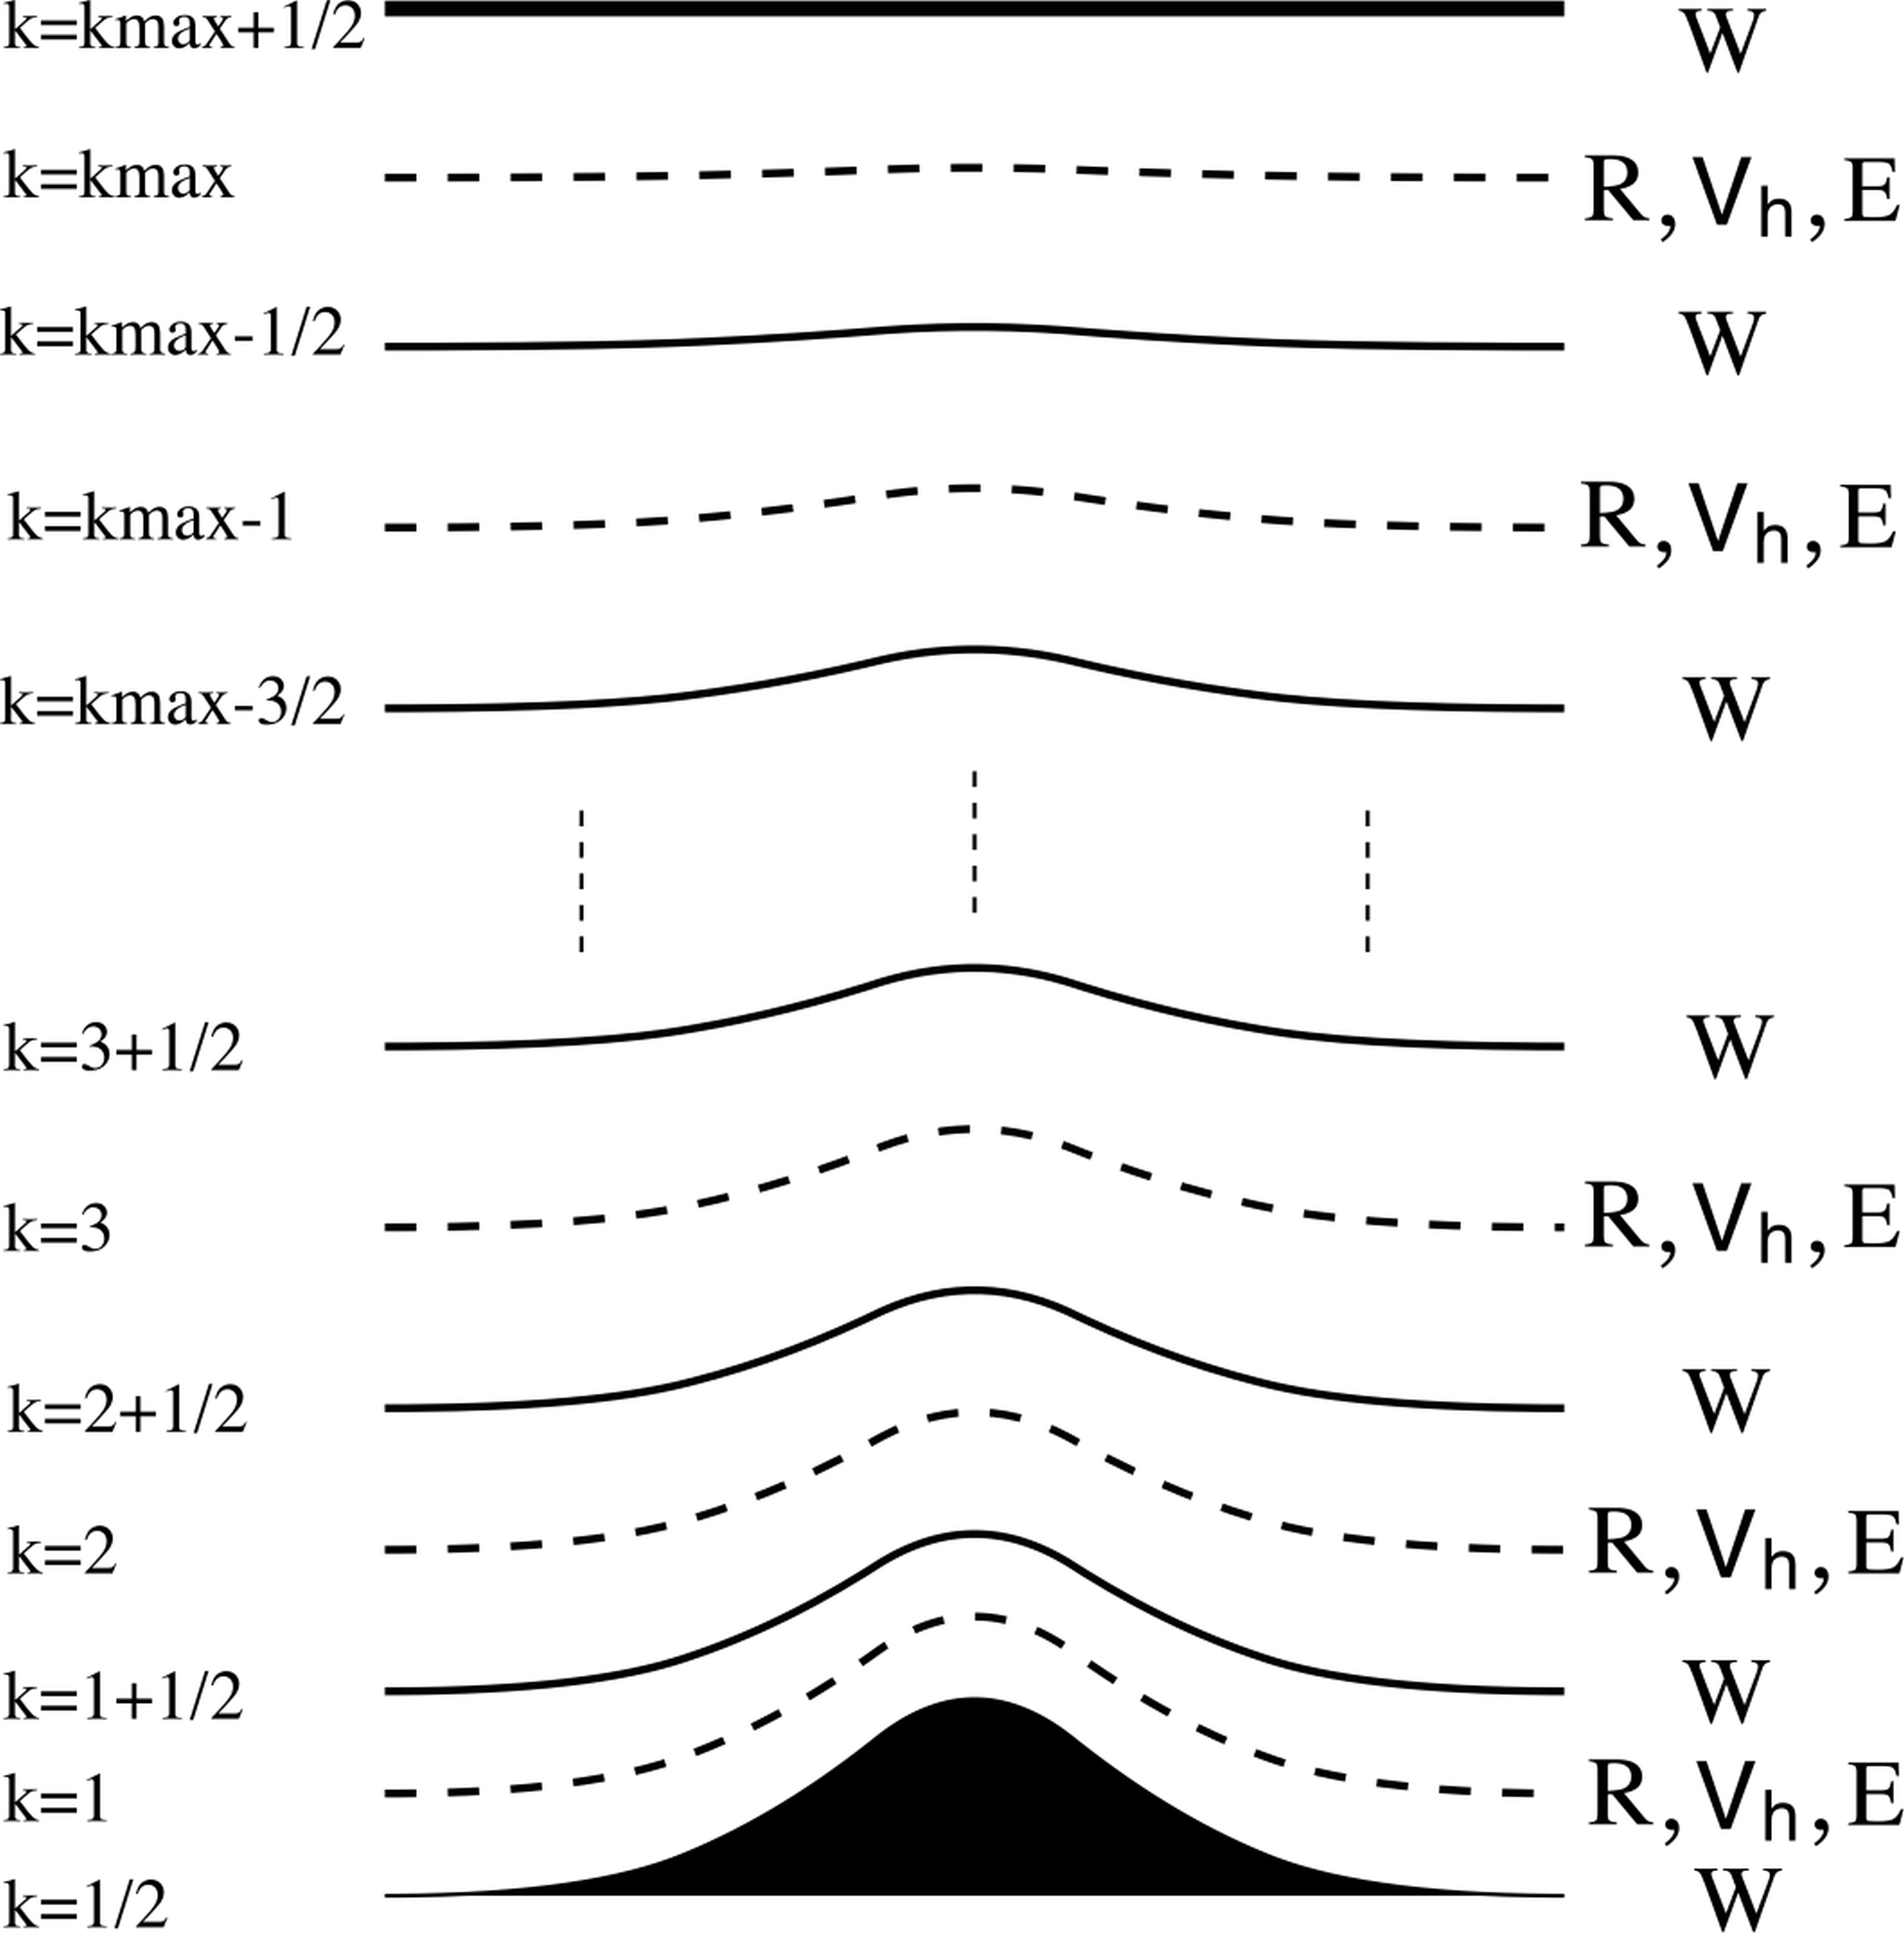
\includegraphics[scale=.4]{./figs/Tomita1-23-1.png}
\caption{Schematic figure of vertical grid configuration.}
\label{f:vert_grid_config}
\end{figure}


One of main solvers is that of the Helmholtz equation, which can be
expressed as
%
\begin{equation}
 - \frac{\partial}{\partial\xi}
 \left[ A^o \frac{\partial(A^i\tilde{W})}{\partial\xi} \right]
 - \frac{\partial(B\tilde{W})}{\partial\xi}
 - C^o \frac{\partial C^i\tilde{W}}{\partial\xi}
 + \alpha D \tilde{W} = S^\text{all}
\label{e:helmholtz_eq}
\end{equation}
%
where
%
\begin{equation}
 \tilde{W} \equiv \frac{{W^* }^{\tau + \Delta \tau}  }{G^{1/2} \gamma^2}
 \left( = {(\rho w)^* }^{\tau + \Delta \tau}\right)
\end{equation}
%
and the coefficients are given as
%
\begin{align}
 A^o &= \frac{1}{G^{1/2}\gamma^2},\\
 A^i &= \gamma^2 h^t,\\
 B   &= \tilde{g}^t, \\
 C^o &= \frac{C_v g}{R_d \gamma^2},\\
 C^i &= \gamma^2, \\
 D   &= \frac{C_v G^{1/2}}{R_d \Delta \tau ^2}.
\end{align}

The source term is given as
\begin{equation}
 S^\text{all} = \frac{C_v}{R_d \Delta \tau^2}
  \left(\frac{\alpha{W^*}^\tau+\Delta \tau S^W}{\gamma^2}
   -\Delta \tau \frac{\partial}{\partial\xi}
   \left[ \frac{1}{G^{1/2}\gamma^2}({P^*}^\tau + \Delta \tau S^P) \right]
-\frac{\Delta \tau}{\gamma^2}({R^*}^\tau + \Delta \tau S^R)g
\right).
\end{equation}
%
\autoref{e:helmholtz_eq} is in discretized form at the level
$k+1/2$:

\begin{align}
&- \left[
    \frac{A^o_{k+1}\left(A^i_{k+3/2}\tilde{W}_{k+3/2}
                    -    A^i_{k+1/2}\tilde{W}_{k+1/2}\right)}
         {\Delta\xi_{k+1}\Delta\xi_{k+1/2}}
   - \frac{A^o_k\left(A^i_{k+1/2}\tilde{W}_{k+1/2}
                -    A^i_{k-1/2}\tilde{W}_{k-1/2} \right)}
         {\Delta\xi_k\Delta_{k+1/2}}
   \right] \nonumber \\
 %
&- \left[
    \frac{\left( c_{k+1} B_{k+3/2}\tilde{W}_{k+3/2}
               + d_{k+1} B_{k+1/2}\tilde{W}_{k+1/2} \right)
    -     \left( c_k B_{k+1/2}\tilde{W}_{k+1/2}
           +     d_k B_{k-1/2}\tilde{W}_{k-1/2} \right)
    }
    {\Delta\xi_{k+1/2}}
  \right] \nonumber \\
 %
&- C^o_{k+1/2} \left[ \frac{\left(c_{k+1} C^i_{k+3/2} \tilde{W}_{k+3/2}
                               + d_{k+1} C^i_{k+1/2} \tilde{W}_{k+1/2}\right)
                         - \left(c_k C^i_{k+1/2}\tilde{W}_{k+1/2}
                               + d_k C^i_{k-1/2}\tilde{W}_{k-1/2}   \right)  }
                         {\Delta \xi_{k+1/2}}\right] \nonumber \\
 %
&+ \alpha D_{k+1/2} \tilde{W}_{k+1/2} \nonumber \\
&= S^{\text{all}}_{k+1/2}
\label{e:helmholtz_eq_discre}
\end{align}
%
where
%
\begin{align}
 S^\text{all}_{k+1/2}
= & \frac{C_v}{R_d \Delta \tau^2}
\left[
 \left(
  \frac{\alpha {W^*}^{\tau}_{k+1/2} + \Delta \tau S^W_{k+1/2}}
       {\gamma_{k+1/2}^2}
 \right)\right. \nonumber\\
&  - \frac{\Delta \tau}{\Delta \xi_{k+1/2}}
\left.
 \left(
  \frac{{P^*}^\tau_{k+1}+\Delta\tau S^P_{k+1}}{G^{1/2}_{k+1}
       {\gamma_{k+1}}^2}
 -\frac{{P^*}^\tau_k + \Delta\tau S^P_k}
       {G^{1/2}_k \gamma_k^2}
 \right)\right. \nonumber\\
&  - g\Delta\tau
\left.
  \left(
   a_{k+1/2}\frac{{R^*}^\tau_{k+1}+\Delta\tau S^R_{k+1}}{\gamma_{k+1}^2}
+  b_{k+1/2}\frac{{R^*}_k^\tau + \Delta\tau S^R_k}{\gamma_k^2}
  \right)
\right]
\end{align}
%
\autoref{e:helmholtz_eq_discre} is a tridiagonal matrix system as follows:
%
\begin{equation}
 \begin{gathered}
  M^L_{k+1/2}\tilde{W}_{k-1/2}
+ M^C_{k+1/2}\tilde{W}_{k+1/2}
+ M^U_{k+1/2}\tilde{W}_{k+3/2}
= S^\text{all}_{k+1/2}, \\
\text{for}  \quad \frac{3}{2} \leq k+\frac{1}{2} \leq k_\text{max} -\frac{1}{2},
 \end{gathered}
\end{equation}
%
where
%


\begin{align}
 M^C_{k+1/2} = & \quad \alpha D_{k+1/2} \nonumber\label{e:M^C}\\
               & + \frac{1}{\Delta\xi_{k+1/2}}
 \left[
   \frac{A^o_{k+1} A^i_{k+1/2}}{\Delta\xi_{k+1}}
 + \frac{A^o_k A^i_{k+1/2}}{\Delta\xi_k}
 - (d_{k+1}-c_k)(B_{k+1/2}+C^o_{k+1/2} C^i_{k+1/2})
 \right],\\
 %
 M^U_{k+1/2} = &
 - \frac{A^o_{k+1} A^i_{k+3/2}}
        {\Delta\xi_{k+1}\Delta\xi_{k+1/2}}
 - \frac{c_{k+1}(B_{k+3/2}+C^o_{k+1/2} C^i_{k+3/2} )}
 {\Delta\xi_{k+1/2}} ,\label{e:M^U}\\
 %
 M^L_{k+1/2} = &
 -\frac{A^o_{k+1}A^i_{k-1/2}}{\Delta\xi_{k+1}\Delta\xi_{k+1/2}}
 +\frac{d_k(B_{k-1/2}+C^o_{k+1/2}C^i_{k-1/2})}{\Delta\xi_{k+1/2}} .\label{e:M^L}
\end{align}
%
If the boundary conditions for $\tilde{W}$ are given at $k=1-1/2$ and
$k_\text{max} + 1/2$, this linear system can be written explicitly as
%

\begin{equation}
\begin{gathered}
  \begin{pmatrix}
 M^C_{1+1/2} & M^U_{1+1/2} & 0 & \cdots & \cdots & \cdots & 0 \\
 M^L_{2+1/2} & M^C_{2+1/2} & M^U_{2+1/2}& 0 & \cdots& \cdots& \vdots \\
  0 & M^L_{3+1/2} & M^C_{3+1/2} & M^U_{3+1/2} & 0 & \cdots & \vdots \\
  \vdots & & \cdots & \cdots & \cdots & & 0\\
  \vdots & \cdots & \cdots & 0 & M^L_{k_\text{max}-3/2}  &M^C_{k_\text{max}-3/2} & M^U_{k_\text{max}-3/2} \\
  0 & \cdots & \cdots & \cdots & 0 & M^L_{k_\text{max}-1/2} &  M^C_{k_\text{max}-1/2} \\
  \end{pmatrix}\\
 \times
  \begin{pmatrix}
   \tilde{W}_{1+1/2}\\
   \tilde{W}_{2+1/2}\\
   \tilde{W}_{3+1/2}\\
   \vdots\\
   \tilde{W}_{k_\text{max}-3/2}\\
   \tilde{W}_{k_\text{max}-1/2}\\
  \end{pmatrix}
  =
  \begin{pmatrix}
   S^\text{all}_{1+1/2} - M^L_{1+1/2} \tilde{W}_{1-1/2}\\
   S^\text{all}_{2+1/2}\\
   S^\text{all}_{3+1/2}\\
   \vdots\\
   S^\text{all}_{k_\text{max}-3/2}\\
   S^\text{all}_{k_\text{max}-1/2} - M^U_{k_\text{max}-1/2}\tilde{W}_{k_\text{max}+1/2}
  \end{pmatrix}
\end{gathered}\label{e:linear_system_explicitly}
\end{equation}
%
Since $A^i$ and $B$ depend on large step values(see \autoref{s:time_integration}), the
compositions of the matrix (\autoref{e:M^C},
\ref{e:M^U}, \ref{e:M^L}, \ref{e:linear_system_explicitly}) are
the updated only at the large step.


\section{Domain decomposition and ``rlevel''}
% Tomita_etal_2008_SIAM Sec3.1

For domain decomposition for parallel computing, \NICAM adopt the
concept of a region-division level, or ``rlevel'', along with the
grid-division level \citep{Tomita:2008jc}.
%
The ten rectangles in \autoref{f:rlevel=0} are the
result of connecting two neighboring triangles of a spherical
icosahedron.
%
This structure is called ``rlevel-0''.
%
For each rectangle, four subrectangles are generated by connecting the
diagonal midgridpoints (\autoref{f:rlevel=1}).
%hu
This structure is called ``rlevel-1''.
%
This process is repeated until the desired number of regions is
obtained.



\begin{figure}[htb]
\centering
\begin{subfigure}{.3\textwidth}
\centering
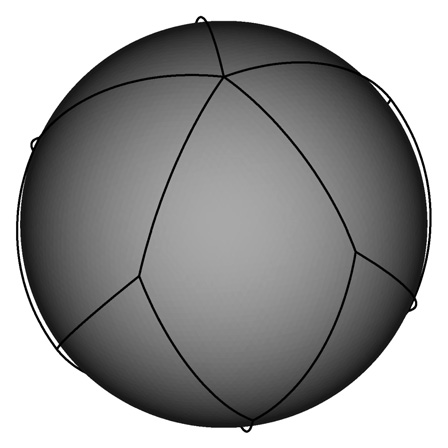
\includegraphics[width=\textwidth]{figs/Tomita_etal_2008_SIAM-8-0.png}
\caption{rlevel=0}\label{f:rlevel=0}
\end{subfigure}
\begin{subfigure}{.3\textwidth}
\centering
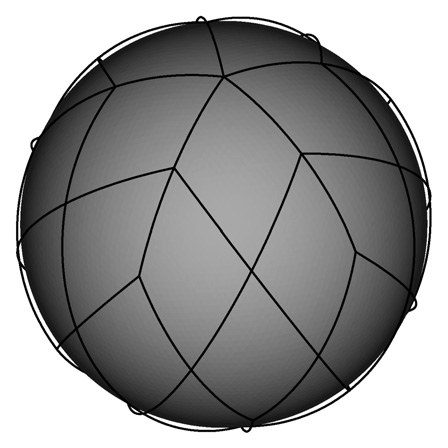
\includegraphics[width=\textwidth]{figs/Tomita_etal_2008_SIAM-8-1.png}
\caption{rlevel=1}\label{f:rlevel=1}
\end{subfigure}
\begin{subfigure}{.3\textwidth}
\centering
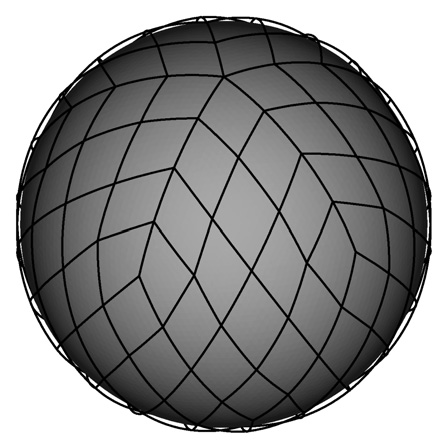
\includegraphics[width=\textwidth]{figs/Tomita_etal_2008_SIAM-8-2.png}
\caption{rlevel=2}
\end{subfigure}
\caption{The method of region division. \citep{Tomita:2008jc}}%
 \label{f:region_division}
\end{figure}



\section{Horizontal data structure}\label{s:horiz_data_structure}

% Tomita_etal_2008_SIAM

As described in \autoref{s:ico_grid_glevel}, the grid elements of an
icosahedral grid are not rectangles.
%
In \NICAM, the shape of the control volume is hexagonal, except for the 12 points
associated with the original icosahedron vertices.
%
Therefore, the icosahedral grid is categorized as an unstructured
grid.
%
However, an icosahedral grid can actually be treated as a structured grid.
%
An example of the grid structure in a region is shown in \autoref{f:normal_region}.
%
The memory of each region in a single layer can be stored as a continuous one- or two-dimensional array.
%
In \autoref{f:normal_region}, the region manages the black gridpoints.
%
The values indicated by the white circles are used only for reference
and are provided from the neighboring regions by communication or memory
copy.
%
The values at the red circles are not used.
%
If the west vertex of a region corresponds to a vertex of the original
icosahedron, the two blue points shown in \autoref{f:normal_region}
have the same values.
%
With this data configuration, the black points cover all the icosahedral
grid points except for the north and south poles.

\autoref{f:pole_region} shows data storage for the pole-region
data.
%
The gridpoint value included in this region is marked by a black
circle.
%
The other values marked by white circles are reference values, provided
by communication or memory copy from the neighboring regular regions.
%
The indices of the reference points are given in clockwise order.
%
The pole regions are managed by the master process.
%
Although this might cause load imbalance in parallel computing, the
ratio of calculation required at the poles to that required in regular
regions is small, and in practice the problem is negligible.

\begin{figure}[htb]
 \begin{subfigure}[t]{.45\textwidth}
  \centering
  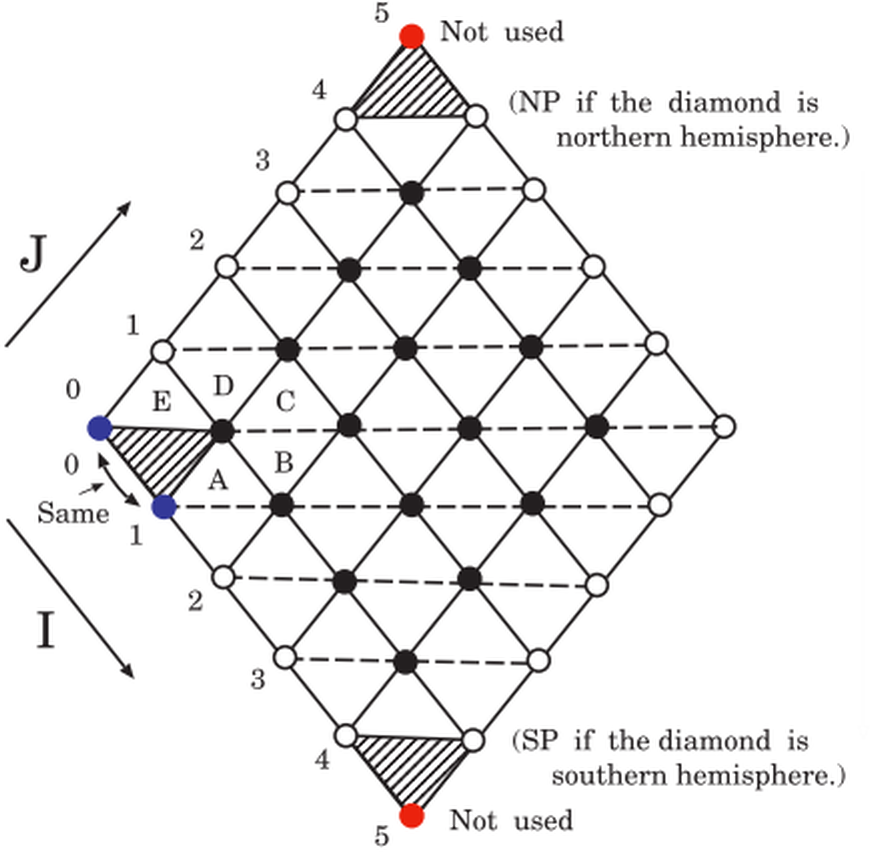
\includegraphics[width=\textwidth]{figs/Tomita_etal_2008_SIAM-9-0.png}
  \caption{Normal region}\label{f:normal_region}
 \end{subfigure}
 \begin{subfigure}[t]{.45\textwidth}
  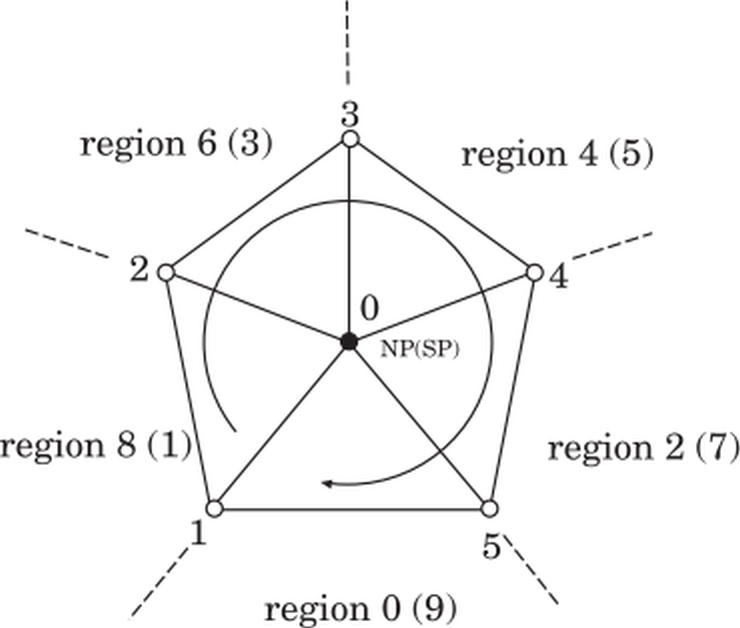
\includegraphics[width=\textwidth]{figs/Tomita_etal_2008_SIAM-9-1.png}
  \caption{Pole region}\label{f:pole_region}
 \end{subfigure}
\caption{Grid structure of a region.\citep{Tomita:2008jc}}
\label{f:grid_structure_of_a_region}
\end{figure}


\section{Parallelization}

%Tomita_etal_2008_SIAM

\NICAM uses MPI for parallel execution.
%
One MPI process manages one or several regions defined in previous
section.
%
For regions managed by the same process, exchanges of boundary values
are done by memory copy, otherwise done by MPI communication.
%
\autoref{f:parallellization} shows a schematic diagram of region
management.
%
In this case, rlevel is 1 and there are 40 regions, managed by 10 MPI
processes.
%
So a single process manages 4 regions, shown by the same color.

\begin{figure}[htb]
\centering
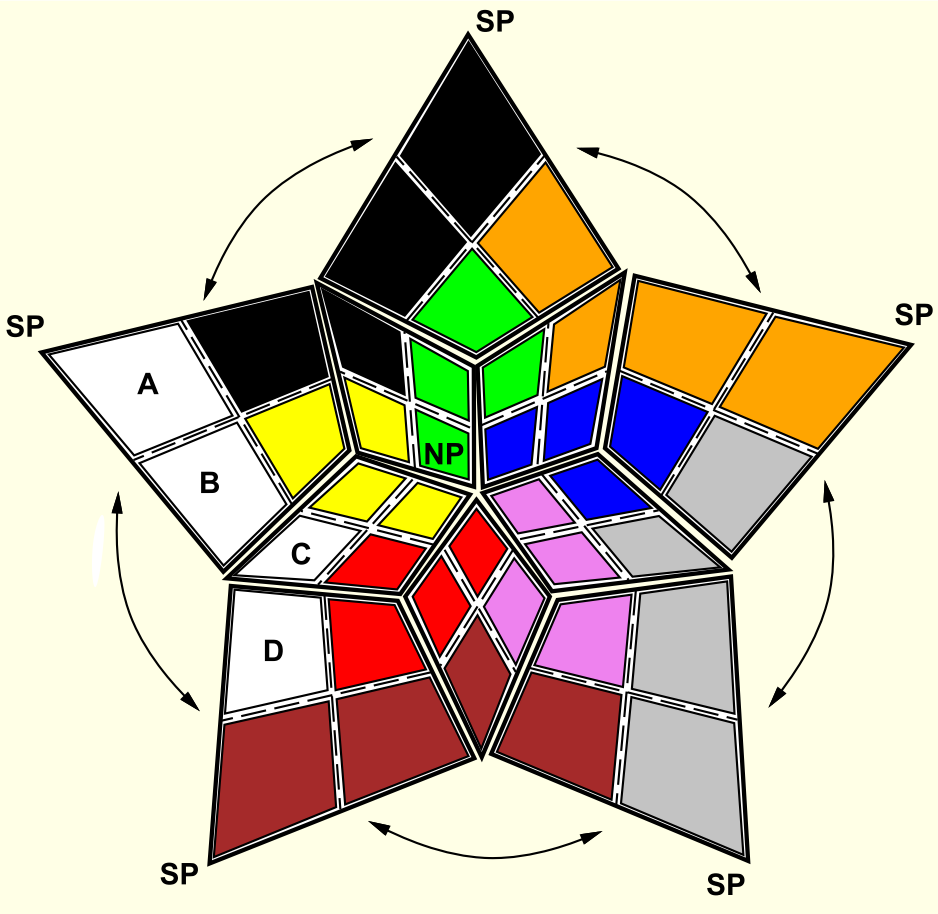
\includegraphics[scale=.7]{figs/Tomita2-10-0.png}
\caption{Schematic figure of parallelization. This figure shows the expansion of region geometry
with rlevel-1.}
\label{f:parallellization}
\end{figure}

\section{Problem size}

As shown in \autoref{s:ico_grid_glevel}, total number of grid points
are defined by glevel.
%
Total grid points $N_g$ is calculated by \autoref{e:N_g}.
%
\begin{equation}
 N_g = 10 \times 4^\text{gl} + 2, \label{e:N_g}
\end{equation}
%
where $\text{gl}$ is glevel. $+ 2$ is corresponding to the pole points.
%
\autoref{t:num_of_grid_points_and_glevel} shows total number of grid points and average
grid point distance for several
glevels.


\begin{table}[htb]
\centering
\caption{Number of grid points and glevel}
\label{t:num_of_grid_points_and_glevel}
\small
\begin{tabular}{|r|r|r|}
\hline
glevel& grid points & average grid interval[\si{\meter]}\\
\hline
 0&  \num{12}&         \num{7142126}\\
\hline
 1&  \num{42}&         \num{3571063} \\
\hline
 2&  \num{162}&        \num{1785432} \\
\hline
 $\cdots$ & $\cdots$& $\cdots$\\
\hline
 8&  \num{655362}&     \num{27899}\\
\hline
 9&  \num{2621442}&    \num{13949}\\
\hline
 10& \num{10485762}&   \num{6975}\\
\hline
 11& \num{41943042}&   \num{3487}\\
\hline
$\cdots$ & $\cdots$& $\cdots$\\
\hline
 13& \num{2684354562}& \num{872}\\
\hline
\end{tabular}
\end{table}


Similary, Total number of regions $N_r$is calculated by \autoref{183551_22Oct17}.
%
\begin{equation}
 N_r = 10 \times 4^\text{rl}, \label{183551_22Oct17}
\end{equation}
%
where $\text{rl}$ is rlevel.
%
\autoref{t:num_of_regions_and_rlevel} shows the relation of rlevel and number of regions.

\begin{table}[htb]
\centering
\caption{Number of regions and rlevel}
\label{t:num_of_regions_and_rlevel}
\small
\begin{tabular}{|r|r|}
\hline
rlevel& number of regions numbers\\
\hline
 0& 10 \\
\hline
 1& 40 \\
\hline
 2& 160 \\
\hline
 3& 640 \\
\hline
 4& 2560 \\
\hline
\end{tabular}
\end{table}

So the number of grid points in a single region (except polar region) $N_p$ is calculated by
\autoref{e:N_p}.
%
\begin{equation}
 N_p = (2 ^ {\text{gl} - \text{rl}} + 2 )^2, \label{e:N_p}
\end{equation}
%
here $+2$ in parentheses denotes the halo grid points.
%
For example, in case glevel is 5 and rlevel is 1, $N_p$ is 324.
%
